% Date: 01.12.15 ------------------ {{{
\marginpar{Date: 01.12.15}

\section{Date: 1.12.15}
  
Def: let y be a function of x 
and $ y^{(n)}(x) = d^{n}y/dx^{n}$ for $n \in \mathbb{N} \left\{ 1, 2, 3, ...\right\} $ 
where F is a given function 

\begin{gather*}
  2xy + x^{2}y' = 1\\ 
  2xy + x^{2}y'-1 = 0
\end{gather*}

This is an ODE, where 

\begin{equation*}
  F(x,y,y') = 2xy + x^{2}y'-1 
\end{equation*}

\section{Date: 1.13.15}
\marginpar{Date: 01.13.15}
  ex: Given f on an interval I find F st 
  $F(x)f'(x)$ for all $x \in I$
  Here F is by def, an antiderivative of f
  on I. we denote F as $\int\limits_{}^{}f(x)dx$.
  All solns $F$ to (1) are of the form $\int\limits_{}^{}f(x)dx+c$, 
  where c is an arbitray constant,
  (1) is an ODE, i.i.,
  \begin{equation*}
    y; = f(x) \iff y'-f(x) = 0
  \end{equation*}
  the latter has the form 
  \begin{equation*}
    f(x,y') = 0 
  \end{equation*}
  A little calc III

  Given $F: \mathbb{R}^n \to \mathbb{R}$, 
  say $\vec{a}=(x_1,...,x_1) \in R^n$, 
  the derivative of F at $\vec{x}$ is 
$$    =F(x)=(F_x1(\vec{x}), F_x2(\vec{x}),..., F_xn(\vec{x})) \in Mat_1xn(R),$$ where 
$$    F_xi(\vec{x})=  \lim_{x \to 0} \frac{F(x_1,..., x_i+h,..., x_n)}{h} $$



  $F_{xi}$ is called the partial derivative of $F$
  with respect to $x_i$. 

  we call $\nabla F = F'$ 
  the gradiant of $F$.

  given $r : I \in R^n$, where I subset R is an integral 
  in R, the derivative of $r$ at t is 

  $$ r'(t) = (x'_1(t), x'_2(t), ... , x'_n(t)),$$ 
  
  $$ r(t) = (x_1(t), x_2(t), ... , x_n(t)),$$

  here $r'(t)$ is a tangent vector to $r$ at 
  $r'(t)$ in $R^n$.

\section{Date: 01.14.15}
\marginpar{Date: 01.14.15}

  Let \( F: \mathbb{R}^n \to \mathbb{R}^m \), say \( x = (x_1, \dots ,
  x_n) \in \mathbb{R}^n  \) and \( F(x) = (f_1) \)

  thrm(Chain Rule). if \( \mathbb{R}^n \): 
% }}}

% Date: 01.26.2015 ---------------------- {{{
\newpage
%\section*{Date: 01.26.2015}
\marginpar{Date: 01.26.15.}
Recall: separable ODE
$$y' = g(x)h(y) \text{ or } \frac{dy}{dx} = g(x)h(y)$$
"separate" the variable as \\
$$\frac{1}{h(y)} y' = g(x) \text{ or }  \frac{1}{h(y)}\frac{dy}{dx} =g(x)$$
$$\int\frac{1}{h(y)} \frac{dy}{dx} dx = \int g(x)dx$$
Now, $y = y(x)$ then by  \\
by change of vars,  \\
$$\int \frac{1}{h(y)} dy = \int \frac{1}{h(y)} \frac{dy}{dx} dx = \int g(x)dx $$
in short,  \\
$$\int \frac{1}{h(y)} dy = \int g(x)dx$$
Now , once these itegrals are evaluated, \\
if possible, then the resolting eqn \\
is one of y on the left and x on the \\
right, which at least implicitly defines  \\
solns y(x) to y' = h(y)g(x). this  \\
resulting eqn may or may not be possible  \\
to solve for y explicitly in terms of x \\

\subsection*{Example}
$x'=kx$, think $x=x(t)$
this is separable; so, 
$$\frac{1}{x} \frac{dx}{dt} = k$$
$$\int \frac{1}{x} \frac{dx}{dt} dt = k \int dt \implies $$
(by change of vars)
$$\int \frac{1}{x} dx = \int \frac{1}{x} \frac{dx}{dt} dt = k\int dt$$
$$\implies ln|x| kt + C \text{, }$$ 
$$\implies |x| = e^{kt+c} = Ce^{kt} \text{, } C=e^c >0$$  
$$\implies x(t) = Ce^{kt}\text{, } C  \neq 0\text{, any }k \in R$$ 

\subsection*{Example}
$T' = k(A-T)$ , $k>0$ \\
this s separable; so,  \\
$$\frac{1}{A-T} \frac{dT}{dt} = k \implies $$
$$\int \frac{1}{A-T} dT = kt + C \implies$$
$$-ln|A-T| = kt + C \implies $$
$$\frac{1}{A-T} = Ce^{kt} \implies$$
$$A-T = Ce^{-Kt} \implies $$
$$T = A-Ce^{-kt}$$


\subsection*{Aside}
substitution (change of vars)
$$\int f(g(x))g'(x)dx = \int f(v)dv$$
$v=g(x)$, or
$$\int f(v)\frac{v}{x} dx = \int f(v)dv$$
% }}}

% Date: 01.27.2015 ---------------------------- {{{
\newpage 
\marginpar{Date: 01.27.15.}
%\section*{Date: 01.27.2015}
  \subsection*{Ex(p.43) 35}
  $$x(t)=ce^{kt} \text{ (form } x=kx)$$
  C14 has a decay rate constant of 
  $$k = -0.0001216$$
  Notice that 
  $$x(0) = C$$
  so, C is called the initial value. \\
  that notation '$x_0$' is used for C \\
  i.e., $x_0 = x(0)$. thus,  \\
  $$x(t)=x_0e^{kt}$$ 
  in \# 35, $x(t) = x_0/6.$ \\
  so, 
  $$\frac{x_0}{6}= x_0e^{kt}$$
  solve for t. thus, 
  $$t=\frac{1}{6}ln(1/6)=\frac{1}{|k|}ln(6)$$
  
  \subsection*{Torricelli's law}
  Think of $x = x(t) \text{ and } h = h(t)$ \\
  we want $x(t)$, say in particular,  \\
  we want t st $x(t) = 0$, so called  \\
  "drain time." \\
  recall \# 35, p.18, that "ground speed" \\
  is given by $|v|=,sqrt{2gx}$ \\
  from "free-fall" a height x.  \\
  in contex, 
  $$\frac{dh}{dt}= \sqrt{2gx}$$
  In "the spout" $V=ah$; so
  $$\frac{dV}{dt}= a\frac{dh}{dt}a\sqrt{cgx}$$
  in the tank 
  $$\frac{dV}{dt}= -a\sqrt{2gx}$$
  let A(x) be the ? cros=sectinal \\
  area of the tank at height x, then  \\
  $$V= \int\limits_{x}^{0}A(t)dt$$
   by ftc(1),
   $$\frac{dV}{dx}= A(x)$$
   by the cain rule
   $$\frac{dV}{dt}= dv/dx dx/dt = A(x)x'$$
   $$a(x)*x' = -a \sqrt{2gx}$$
   i.e.
   $$x'A(x)= -a\sqrt{2gx}$$
   which is a separable ODE. thus
   $$\frac{A(x)}{\sqrt{x}} dx = -a\sqrt{2g} \implies$$
   (int w.r.t t and $\Delta$ vars)
   $$\int \frac{A(x)}{\sqrt{x}} dx= -at\sqrt{2g}$$
   % }}}

% Date: 01.29.2015 -------------------------- {{{ 
\newpage
\marginpar{Date: 01.29.15}
\section{Date: 01.29.2015}
  
  \subsection*{Ex (p.45) \# 59} 
  revolve \(x^2 = by\) about y-axis \\	
  depth is 4ft at noon, \(y(0) = 4\)
  \[a = \pi r^2\]
  depth is 1ft at 1pm same day  \\
  Recall: \(\int y^{-1/2} A(y)dx= -8at\) in ft and s. \\
  thus, by torciullis law,  \\
  \[-8 \pi r^2t = \pi b \int y^{1/2}dy \implies \]
  \[-8r^2t = \frac{2b}{3} y^{3/2} + C\]
  \[y(0) = 4 \implies C = -16b/3\]
  \[\therefore\]
  \[\frac{2b}{3} y^{3/2}= \frac{16b}{3}-8 r^I 2t\]
  Now, in 3600s (1hr), y=1, i.e., y(3600) = 1, 
  \[\frac{2b}{3} = \frac{16b}{3}-8r^2(3600)\]
  \[r^2 = \frac{14b}{3*8*3600} = \frac{7b}{12*3600} \implies \]
  \[r = \frac{1}{60} \sqrt{\frac{7b}{12}}\]
  Drain time \(t_0\) is 
  \[0 = \frac{16b}{3} - 8r^2t_0 \implies t_0 = \frac{2b}{3r^2}\]
  Now, in particuler, if  \\
  \( y = 4 \), then the radius  \\
  of \( A(y) \) is 2, i.e., \( x = 2 \). \\ 
  Thus,
  \[x^2 = by \implies 4 = 4b \implies b=1 \therefore\]  
  \[r = \frac{1}{60} \sqrt{\frac{17}{12}}   \text{ \& } t_0 =
  \frac{2}{3r^2}\]
  % }}}

% Date: 02.02.2015 ---------------------------- {{{
\newpage
\marginpar{Date: 02.02.15}
\section{Date: 02.02.2015}
  Thrm  existence - uniqueness thrm, \( \exists \text{!thrm} \)  \\	
  If \( f: D, \subseteq \mathbb{R}^2 \to  \mathbb{R} \) and \( f_y : D_2
  \subseteq \mathbb{R}^2 \to \mathbb{R}\) \\
  are cts on \( R = (a, b) x (c, d) \) and \( x_0, y_0) \in R\) and \\
  then these exist an interval I st \( x_0 \in I\), \( I \subseteq (a,
  b)\) and \\
  the initial value problem
  \[ \frac{dy}{dx} = f(x, y) \text{ and } y_0 = y(x_0)\]
  has a unique \( y = y(x) \) for all \( x \in I\). \\ 

  %pic
  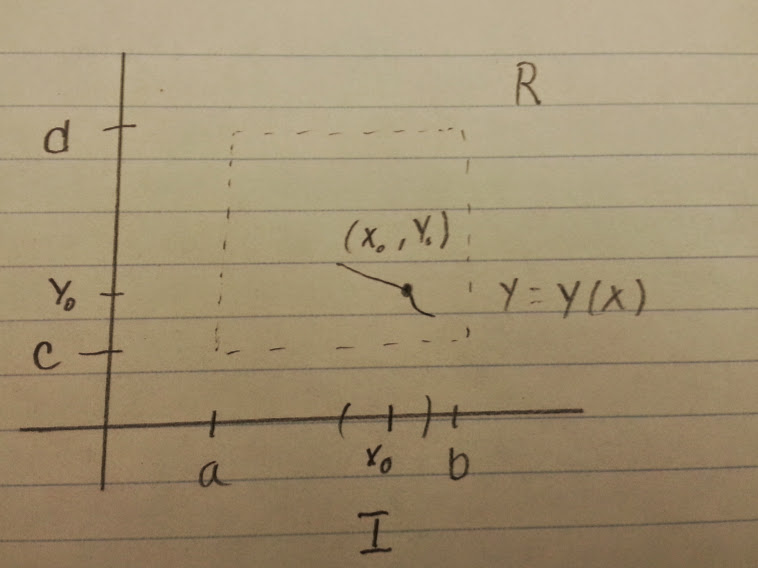
\includegraphics[scale=.45]{pic1}
  
  \begin{tikzpicture}[scale=.6]
  
     
    %\draw[step=1cm, teal, very thin] (0,0) grid (10,10); % Grid lines
  
    \draw[thick, ->] (-1,0) -- (10,0) % + x axis line
    	node[anchor=north west] { \( x \) }; % x axis lable 
  
    \draw[thick,->] (0,-1) -- (0,10) % + y axis line 
    	node[anchor=south east] { \( y \) }; % y axis lable

    \draw[very thick, red]
    (4,5)  to [out=60, in=180] (6,2.99) to [out=0, in=128] (8,2.3); 

    \draw[fill] (6,3) circle [radius=2pt] % dot in top right corner
    	node[above right]  { \( (x_0, y_0) \)}; % lable (10,10) 

    \draw[thick,  dashed] 
    (2,2) -- (2,9) -- (9,9) node[above right] { \( R \)} --
    (9,2) -- (2,2);
  
    \draw[thick]
    (-.5,9) node[left] { \( d \)} -- (.5,9);

    \draw[thick]
    (-.5,3) node[left] { \( y_0 \)} -- (.5,3);

    \draw[thick]
    (-.5,2) node[left] { \( c \)} -- (.5,2);

    \draw[thick]
    (2,-.5) node[below] { \( a \)} -- (2,.5);
   
    \draw[thick]
    (9,-.5) node[below] { \( b \)} -- (9,.5);

    \draw[thick]
    (6,-.5) node[below] { \( x_0 \)} -- (6,.5);

    \node [red, below] at (11,3) { \( y=y(x) \)};
    
  \end{tikzpicture}
  \\[5mm]

  \[ R = (a, b)x(c, d)\]
  \[ = {(x, y) \in R^2 | a < x < b \text{ \& }  c < y < d } \]
  The \( \exists \text{! thrm} \) is a "local" result, local \\
  to \(x_0\), move precisely, it just sups that there is a unique soln in I \\
  not necessarily outside of I. \\

  \subsection*{Ex(p.29) \# 27}
  
  \[ y' = s \sqrt{y} \text{ \& } y(0) = 0\]
  consider 
  \[ y(x) = \left\{
  \begin{array}{l l}
	0 & x\leq c \\
	(x-c)^2 &  x \geq c
  \end{array}\right. \]
  which is ctn on \( \mathbb{R} \)  \\
  notice that both parts  \\
  y(x) satisfy the initial value problem if \\
  \( c \geq 0\) Note: 

  % pic
  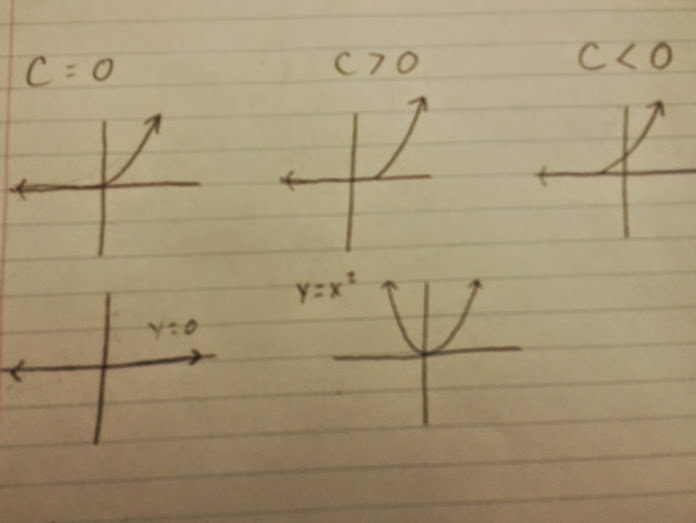
\includegraphics[scale=.45]{pic2}

  Notice that
  \[ f(x, y) = 2\sqrt{y} \text{ \& } f_y(x, y) = \frac{1}{ \sqrt{y}}\]
  which is cts on \( R = \{ (x, y) \in R^2 |  y > 0\}\)

  % pic 
  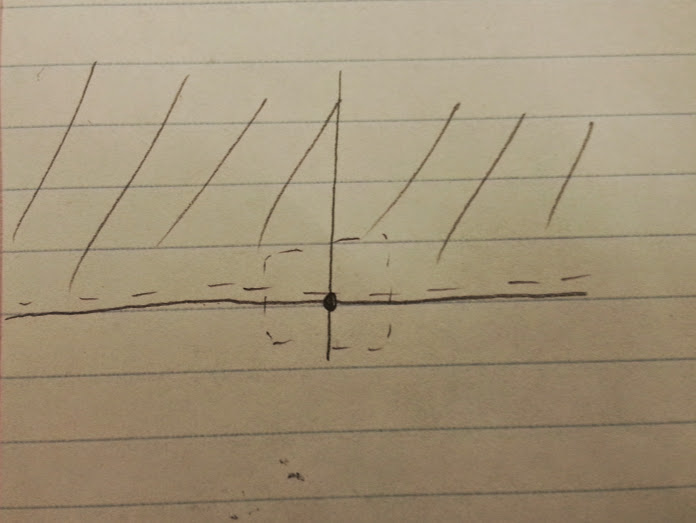
\includegraphics[scale=.45]{pic3}

  notice that (0, 0) is not in R, not \\
  "interior" to R. \( \therefore \exists \text{! thrm}\) does not apply
  \\
  Notice that if \( y = f(x) \) is a soln to \\
  an ODE on a interval I  \\
  then so is \( y = f(x-c)\) a soln to  \\
  the ODE on \( I - c =\{ x \in R | x + c \in I\}\).  \\
  % }}} 

  % Date: 02.03.2015 ------------------- {{{
  \newpage 
\marginpar{Date: 02.03.15.}
%\section{Date: 02.03.2015}
  \subsection*{ ex p.28 }
  15. \( y' = \sqrt{x-y} \text{ ,  } y(2) = 2 \),  no \\
  16. \( y' = \sqrt{x-y} \text{ ,  } y(2) = 1 \),  yes \\
  here \( f(x, y) = \sqrt{x-y}\) , which has \\
  cts iff  \( x-y \geq 0 \iff x \geq y\) \\ 
  \( f_y(x, y) = - \frac{1}{2\sqrt{x-y}}\),  which is cts \\
  on \( \{ (x,y) \in \mathbb{R}^2 \text{ | } y<x \}\). \\
  \subsection*{ Notes \\ } 
  Def A first order linear ODE \\
  has the form
  \[ \text{ (1) } y' + p(x)y = q(x)\] 
  where p \& q are cts on some interval \( \mathcal{I}\). \\
  Notice that if \( q(x) = 0\) then (1) is \\	
  separable. \\	  
  Key observation: the left side of \\
  (1) resembols the product rule. \\
  this motivates a question: Is there \\
  a cst I(x), say on the interval \( \mathcal{I}\),  \\
  st  \\
  (1') \( y'I(x) + yp(x)I(x) = q(x)I(x)\) ,  \\
  where the left side of (1') is the dirivative  \\
  of a product? \\

  if there is such an I(x)  \\
  then  \\
  (2) \( I'(x) = p(x)I(x)\). \\
  put \( v = I(x)\), then (2) becomes  \\
  \[ v' = p(x)v\]
  which is separable. thus \nonumber\\
  \[ \frac{v'}{v} = p(x) \implies\]
  \[ \int \frac{1}{v}dv = \int p(x)dx \implies\]
  \[ \ln|v| = \int p(x)dx + C \implies \]
  \[ |v| = e^{\int p(x)dx + C} = Ke^{\int p(x)dx}\]
  where \( k > 0 \therefore\)
  \[ v = Ke^{\int p(x)dx} \text{ , } K \neq  0\]
  Def. the intergrating factor of 
  \[ y' + p(x)y = q(x) is \]
  \[ I(x) = e^{\int p(x) dx }\]
  Finally, from (1') 
  \[ (yI(x))' = q(x)I(x) \implies \]
  \[ yI(x) = \int q(x)I(x)dx \implies\] 
  \[ \boxed{ y = \frac{1}{I(x)} \int q(x)I(x)dx}\]
  % }}}
 
  % Date: 02.04.2015 -------------------------- {{{
  \newpage
\marginpar{Date: 02.04.15.}
%\section{Date: 02.04.2015}

\subsection*{Single Tanking Problem}
 \( c_i\) = concentration coming into the tank (constant) \\
 \( r_i\) = rate of flow into the tank (constant) \\
 \( c_0(t)\) = concentration coming out of the tank \\
 \( r_0\) = rate of flow out of the tank (constant) \\
 \( x(t) \) = amount of salute in tank at time t \\
 \( V(t)\) volume of tank at time \( t\) \\[5mm] 
 Units: \\
 Concentration = \( \frac{ \text{ amount of solute }}{ \text{ unit
 valume	 }}\) \\ 
 Rate = \( \frac{ \text{ valume }}{ \text{ unit time }}\) \\	 
 amount = (concentration)(rate)(time) \\[5mm]
 Notice that the rate of change fo the volume is constant and  \\
 is \( m = r_i - r_0\); where, \( V(t) = (r_i - r_0)t + V_0 = mt +
 V_0\), where \( V_0 = V(0)\) \\
 For a small \( \Delta t\)\nonumber\\
 \( x(t + \Delta t) = x(t) + \text{ amount in = amount out over time }
 \Delta t\) \\[5mm]
 amount in over \( \Delta t = c_i r_i \Delta t\); \\
 amount out over \( \Delta t \approx c_0(t) r_0 \Delta t\). \\
 thus,  \\
 \[ \Delta x = x(t + \Delta t) - x(t) \approx (c_i r_i - c_0(t)r_0) \Delta
 t \implies \]

 \[ \frac{\Delta x}{\Delta t} \approx c_i r_i - c_0 (t) r_0\]
 this suggest that  \\
 \[ \frac{dy}{dx} = c_i r_i - c_0 (t) r_0\]
 Now\nonumber\\
 \[ c_0(t) = \frac{x(t)}{V(t)} \implies \]
 \[ \frac{dx}{dt} = c_ir_i = \frac{x(t)}{V(t)}r_0\]
 which is a 1st order linear ODE. \\
 more consiely, put \( x' = \frac{dx}{dt}\) and \\
 \( x= x(t) \), then  \\
 \[ \boxed{x' + \frac{r_0}{V(t)}x = c_ir_i}\]
 Recall that \( V(t) = mt + v_0 \text{ , } m = r_i - r_0\); so,  \\
 \[ x' + \frac{r_0}{mt + v_0} x = c_ir_i\] 
 Here  \\
 \[ p(t) = \frac{r_0}{mt + V_0} \implies\]
 \[ \int p(x) dx = \frac{r_0}{m} ln (mt + V_0) + C\] 
 where in context, \( V(t) > 0\). Choose, of ease, \\ 
 \( C = 0\), then \\
 \[ I(t) = e^{\int p(t)dt} = (mt + V_0)^{r_0/m}\]
 So,  \\
 \[ x'(mt + V_0)^{r_0/m} + r_0(mt + V_0)^{r_0/m -m } = c_ir_i(mt +
 V_0)^{r_0/m} \implies \]
 \[ (x(mt + V_0)^{r_0/m})' = c_ir_i+(mt + V_0)^{r_0/m} \implies\]
 \[ x(mt+V_0)^{r_0/m} = c_ir_i \int (mt +V_0)^{r_0/m}dt\]
 If \( r_0/ m = -1 \) then \( r_0 = -m = -r_i + r_0\) \\
 \( \implies r_i = 0 \), which is not of intrest in \\ 
 context ("mixing").  Thus, if \( r_0/m \neq -1\) \\
 then 
 \[ \int (mt + V_0 )^{r_0/m}dt = \frac{1}{m}(mt + V_0)^{r_0/m +
 1}\frac{m}{r_0 + m} + C\]
 \[ = \frac{1}{r_i}(mt + V_0)^{r_i/m} + C\]
 \[ \therefore\]
 \[ x(mt + v_0)^{r_0/m} = c_i(mt + V_0)^{r_i/m } + C\]
 at \( t = 0\)
 \[ x_0V_0^{r_0/m} = c_iV_0^{r_i/m} + C \implies\]
 \[ C = c_iV_0^{r_i/m} - x_0V_0^{r_0/m}\]
 \[ = V_0^{r_0/m}(c_iV_0 - x_0)\]
 thus, 
 \[ x(mt + V_0)^{r_0/m} = c_i(mt+V_0)^{r_0/m} + V_0^{r_0/m}(c_iV_0 -x_0\]
 \[ \implies x = c_i(mt + V_0) + (c_iV_0 - x_0)
 (\frac{V_0}{mt+V_0})^{r_0/m}\]

 \begin{empheq}[box=\fbox]{align}
	x = c_iV + (c_iV_0 - x_0)
	\bigg(\frac{V_0}{V}\bigg)^{r_0/(ri-r_0)} \nonumber \\
	\text{ where } x = x(t) \text{ \& } V = (r_i-r_0) t + V_0
	\nonumber 
 \end{empheq} 

 %\[ \boxed{x = c_iV + (c_iV_0 - x_0) (\frac{V_0}{V})^{r_0/(ri-r_0)} \\
 %\text{ where } x = x(t) \text{ \& } V = (r_i-r_0) t + V_0}\]

 % }}}  

%\section{Date: 02.05.2015 } 

 % Date: 02.09.2015 ------------------------ {{{
 \newpage 
\marginpar{Date: 02.09.15.}
\section{Date: 02.09.2015}
  1.6 Substitutions in ODEs \\
  Consider a slope field  \\
  \[ \text{ (1) } \frac{dy}{dx} = f(y, x)\]
  i.e., a 1st order normal ODE. If
  \[ \alpha (x, y)\]
  appers in (1), then we are compelled  \\
  to make the substitution  \\
  \[ v = \alpha (x, y)\]
  ("alpha" for auxillary variable) \\
  By the calc III chain rule\nonumber\\
  \[ \frac{dv}{dx} = \frac{\partial\alpha}{\partial x} \frac{dx}{dx} + \frac{\partial
  \alpha}{\partial y} \frac{dy}{dx}\]
  
  \[ = \alpha_x + \alpha y \frac{dy}{dx}\]
  
  If \( v = \alpha (x, y) can be soved \) \\
  for y in terms of x and v, say  \\
  \[ y = \beta(x, v) \] \\
  then from (1), we have that  \\
  \[ \frac{dv}{dx} = \alpha_x + \alpha_y \frac{dy}{dx} = \alpha +
  \alpha_y f(x, y) \]
  where, 
  \[ \boxed{ \frac{dv}{dx} = \alpha_x + \alpha f(x, \beta(x, v))}\]

  which is a new ODE with dependent variable v
  and independent variable x. 
  \subsection{ex}
  \[ \frac{dy}{dx} = f(x, y , ax+by+c\]
  put 
  \[ v + d(x, y) = ax + by + c\]
  then 
  \[ \frac{dv}{dx} = a + b \frac{dy}{dx}\]
  thus, 
  \[ \frac{dv}{dx} = a + b \frac{dy}{dx} = a + b f(x, y, ax + by +c)\]
  \[ \implies \boxed{\frac{dv}{dx} = a + b f(x, (v-ax-c)/b, v)}\]
  where 
  \[ y = \beta (x, v) = \frac{v-ax-c}{b} \text{ , } b \neq 0\]

  \subsection{p.74 16}
  \[ y' = \sqrt{x+y+1}\]
  \[ v = x + y + 1 \implies y = v - x - 1 \text{ \& } \]
  \[ \frac{dv}{dx} = 1 + \frac{dy}{dx} \implies \]
  \[ \frac{dv}{dx} = \sqrt{v} + 1 \text{ (separable) }\]

  Def. A first order normal homogenous 
  ODE has the form 
  \[ \frac{dy}{dx} = f(y/x)\]

  \subsection{Ex}
  \[ y' = \frac{xy}{x^2 + y^2}\]
  In general, put 
  \[ v = \alpha (x, y) = y/x \text{ (slope) }\]
  so, \( y = xv\) implies that 
  \[ f(v) = f(y/x) = \frac{dy}{dx} = v + x \frac{dv}{dx} \implies \]
  \[ x \frac{dv}{dx} = f(v) - v \text{ (separable) }\]
  \[ \frac{1}{f(v) -v} \frac{dv}{dx} = \frac{1}{x} \implies \]
  \[ \int \frac{1}{f(v) -v} dv = \ln |x| + c\]

  \subsection{Ex (Revisited)}

  \[ y' = \frac{xy}{x^2 + y^2} = \frac{y/x}{1 + (y/x)^2} , v = y/x
  \implies \]
  \[ \int \frac{1}{\frac{v}{1 + v^2} -v}dv = \ln |x| + c \implies \]
  \[ - \int \frac{1 + v^2}{v^3}dv = \ln |x| + c \implies \dots \]
  % }}}

  % Date: 02.10.15 ------------------- {{{
  \newpage 
\marginpar{Date: 02.10.15}
\section{Date: 02.10.2015}
  Thrm. If \( p(x, y) = \sum a_{i_1 i_2} x^{i_1} y^{i_2} \) and \\
  \( Q(x, y) = \sum a_{j_1 j_2} x^{j_1} y^{j_2} \) are polynomials \\
  over \( \mathbb{R} \), then if there is a \( k \in \mathbb{Z}^+ \) st
  for all \( i_1, i_2, j_1, j_2,  \)
  \[ i_1 + i_2 = d = j_1 + j_2 \]
  then \( p(x, y)y'=Q(x, y)  \) is a 1st order linear \\
  homogenous ODE.\\
  Proof. notice that 
  \[ y' \sum a_{i_1 i_2} x^{i_1} y^{i_2} = 
  \sum a_{j_1 j_2} x^{j_1} y^{j_2} \implies \]

  \[ \frac{1}{x^d} y' \sum a_{i_1 i_2} x^{i_1} y^{i_2} = 
  \frac{1}{x^d} \sum a_{j_1 j_2} x^{j_1} y^{j_2} \implies \]

  \[ y' \sum a_{i_1 i_2} \frac{y^{i_2}}{x^{d-i_1}} =
   \sum b_{j_1 j_2} \frac{y^{j_2}}{x^{d-j_1}} \implies\]
   
   \[ y' \sum a_{i_1 i_2} (\frac{y}{x})^{i_2} =
   \sum b_{j_1 j_2} (\frac{y}{x})^{j_2}  \implies\]
   
   \[ y' =  \frac{\sum a_{i_1 i_2} (\frac{y}{x})^{i_2}}{\sum b_{j_1 j_2} (\frac{y}{x})^{j_2} }\]
   which is hom. endproof

   Def. (i) deg \( a_{i_1, i_2 ...i_n} x_1^{i_1}, x_2^{i_2}, \dots
   x_n^{i_n} = \sum_{k=1}^{n} i_{k i}\)

   (ii) deg \( ((p(x_i)) \)
   
   where \( p(x_1, x_2, \dots , x_n = \sum a_{i_1 i_2 \dots i_n}
   x_1^{i_1} x_2^{i_2} \dots x_n^{i_n} \)

   \subsection{ex p.74 2} 

   \[ 2xyy' = x^2 +2y^2 \implies  \]
   \[ y' = (\frac{1}{2} \frac{1}{y/x} + 2(y/x)) \text{ , } v = y/x
   \implies \]
   \[ y = vx \implies y' = v + xv' \text{ \& } xv' +v = \frac{1}{2v} +v
   \implies \]
   \[ v' = \frac{1}{2xv} \text{ (separable) } \implies  \]
   \[ vv' = \frac{1}{2x} \implies \]
   \[ \int v dv = \frac{1}{2} \int \frac{1}{x} dx = \frac{1}{2} \ln |x|
   \implies \]
   \[ \frac{v^2}{2} = \frac{1}{2} \ln |x| + c \implies  \]
   \[ v^2 = \ln |x| + c \implies  \]
   \[ v = +- \sqrt{ \ln |x| + c} \implies \]
   \[ \frac{y}{x} +- \sqrt{\ln |x| + c} \implies  \]
   \[ y = +-x \sqrt{\ln |x| + c} \]
   Def. A first order (normal) \\
   berelli ODE has the 
   \[ y' +yp(x) = y^nq(x) \]

   side note(good book) Asmov PDE 
\section{Date: 02.11.2015}
  Recall: Bernulli ODE
  \[ y' + yp(x) = y^n q(x) \]
  put \( v = y^m \) then
  \[ \frac{dv}{dx} = my^{m-1} \frac{dy}{dx} \implies \]
  \[ my^{m-1} \frac{dy}{dx} + my^m p(x) = my^{m+n-1}  q(x) \implies \]
  % needs perp sign
  \[ \frac{dv}{dx} vmp(x) = my^{m+n-1}  q(x)\]
  want: \( m+n-1=0 \). this requires \\
  that \( m = 1-n \). \( \therefore v=y^{1-n}\) reduses \\
  a bernoulli ODE to a 1st order linear ODE. \\

  \subsection{p.74 25}
  \[ y^2(xy'+y)(1+x^4)^{1/2} = x \]
  \[ \implies (xy^2y' + y^3) \sqrt{1+4x} = x\]
  \[ \implies xy^2y' \sqrt{1+x^4} + y^3 \sqrt{1+x^4} = x \]
  \[ \implies y' \sqrt{1+x^4} + y \frac{ \sqrt{1+x^4}}{x} = y^{-2} \]
  \[ \implies y' +y \frac{1}{x} = y^{-2} \frac{1}{ \sqrt{1+x^4}} \]
  put \( v = y^3 \) then 
  \[ \frac{dv}{dx} = 3y^2 \frac{dy}{dx} \implies \]
  \[ 3y^2y' + \frac{3y^3}{x} = \frac{3}{ \sqrt{1+x^4}} \implies \]
  \[ v' + \frac{3v}{x} = \frac{3}{ \sqrt{1+x^4}} \text{ (linear) } \]
  Here \( p(x) = 3/x \); so\nonumber\\
  \[ I(x) = e^{\int p(x)dx} = e^{3\ln |x|} = x^3 \]
  Thus, 
  \[ v'x^3 ' + v3x^2 = \frac{3x^3}{ \sqrt{1+ x^4}} \implies \]
  \[ (vx^3)' = \frac{3x^3}{ \sqrt{1+x^4}} \implies \]
  \[ vx^3 = 3 \int \frac{x^3}{ \sqrt{1 + x^4}}dx = 
  \frac{3}{4} \int w^{-1/2} dw\]
  \[ \frac{3}{4} \frac{2}{1}w^{1/2} + c\]
  \[ \frac{3}{2} ( \sqrt{1+x^4} + c \]
  \[ w = 1+x^4  \]
  \[ w' = rx^3 \]
 % need stuff

 \[ y^3 = \frac{3}{2} ( \frac{ \sqrt{1+x^4} + c}{x^3}) \implies  \]
 \[ y =  (\frac{3}{2} ( \frac{ \sqrt{1+x^4} + c}{x^3}))^{1/3}\] 

 % }}}

 Exam 1 
 1. Given an ODE and a soln to it, verify it is a soln, then find a
 particular soln givin an initial cond.

 2. Given a description of an ODE, write down the ODE. 

 3. Dropping ball from some h, find , ground time and speed.

 4. high jump on earth given, find high jump on jupiter. 

 5. (a) solve ODEs 
 
(b) 

one is separable and the other is linear or bornulli

6. Torricelli problem. 
